In this section, we simulate the implementation of both the control-aware CALLS method and a standard ``control-agnostic'' scheduling methods for various low-latency control systems over a simulated wireless channel. We point out the low-latency based scheduling/assignment approaches of both methods being compared are identical, with the distinguishing features being the dynamic control-aware packet delivery rates incorporated in the CALLS method. In doing so, we may analyze the performance of the control-aware design outlined in the previous section relative to a standard latency-aware approach in terms of, e.g., number of users supported with fixed latency threshold or best latency achieved with fixed number of users. As we are interested primarily in low latency settings that tightly restrict the communication resources, we consider two standard control systems whose rapidly changing state requires high sampling rates, and consequently a communication latency on the order of milliseconds. The parameters for the simulation setup are provided in Table \ref{tab_simulation}. The packet delivery rate function $q(\bbh,\mu,\bbsigma)$ is computed using the standard AWGN noise curves for wireless channels. The transmission time $\tau(\mu,\bbsigma)$ is computed in the simulations using the associated data rates of an MCS in Table \ref{tab_mcs} for a 100 byte packet and overhead (e.g. TFs) of the 802.11ax specifications. The latency overhead for this setting amounts to approximately $\tau_0 \approx 100 \mu$s.
%
\begin{table}
\begin{tabular}{ l | l } \hline
  Channel model & IEEE Model E (indoor) \cite{liu2014ieee} \\
  Sensor to AP distances & Random (1 to 50 meters)\\
  Transmit power & 23 dbm \\
  Channel bandwidth & 20 MHz \\
  RU sizes & 2, 4, 8, 20 MHz \\
  \# of antennas at AP & 2 \\
  \# of antennas at sensors & 1 \\
  MCS options & See Table \ref{tab_mcs} \\
  State sampling period & 10 ms \\
  \hline
\end{tabular}
\caption{Simulation setting parameters.}
\label{tab_simulation}
\end{table}
%

\subsection{Inverted pendulum system}

\begin{figure}
%% -*- Mode: LaTeX Memoir; tab-width: 4;

%% InvertedPendulum.tikz    Inverted Pendulum
%% Draw an inverted pendulum using PGF/TikZ
%% MAIN FILE: ../../TikZGallery.tex
%% Created by Dazhi Jiang, 2011-02-01 16:49:22 +0000 (Tue,  1 Feb 2011)
%% Copyright (c) 2011 Dazhi Jiang. All Rights Reserved. 

%% TextMate Settings
%!TEX root = ../../TikZGallery.tex

\newif\ifpendulumcolored
\pendulumcoloredtrue

\ifpendulumcolored

\tikzset{%
	interface/.style={
		% The border decoration is a path replacing decorator. 
		% For the interface style we want to draw the original path.
		% The postaction option is therefore used to ensure that the
		% border decoration is drawn *after* the original path.
		postaction={draw, decorate, decoration={border, angle=-45,
					amplitude=0.3cm, segment length=2mm}}},
	helparrow/.style={>=latex', blue, thick},
	% helparrow/.style={>=latex', draw=blue, fill=blue, very thick},
	helpline/.style={thin, black!90, opacity=0.5},
	force/.style={>=stealth, draw=blue, fill=blue, ultra thick},
	cart/.style={draw = black,%fill = black!40,%
				top color = green!5,%
				bottom color = green!40,%
				% pattern=horizontal lines gray,%
				},
	pendulum/.style={draw = black,% fill = black!25,%
					left color = red!10,%
					bottom color = red!40,%
					% pattern=horizontal lines gray,%
					},
	ground/.style={fill=brown!20},
	inner wheel/.style={fill=black!50},
	outer wheel/.style={thin,double = black!75,double distance = 0.6mm,black},
	wheel shadow/.style={thin,fill = black!70,path fading = south},
	xycoord/.style={<->, thick, black!50},
}

\else

\tikzset{%
	interface/.style={
		% The border decoration is a path replacing decorator. 
		% For the interface style we want to draw the original path.
		% The postaction option is therefore used to ensure that the
		% border decoration is drawn *after* the original path.
		postaction={draw, decorate, decoration={border, angle=-45,
					amplitude=0.3cm, segment length=2mm}}},
	helparrow/.style={>=latex', blue, thick},
	% helparrow/.style={>=latex', draw=blue, fill=blue, very thick},
	helpline/.style={thin, black!90, opacity=0.5},
	force/.style={>=stealth, draw=blue, fill=blue, ultra thick},
	cart/.style={draw = black!80,%fill = black!40,%
				top color = black!10,%
				bottom color = black!40,%
				% pattern=horizontal lines gray,%
				},
	pendulum/.style={draw = black!80,% fill = black!25,%
					left color = black!10,%
					bottom color = black!40,%
					% pattern=horizontal lines gray,%
					},
	ground/.style={fill=black!20},
	% ground/.style={fill=black!20},
	inner wheel/.style={fill=black!30},
	outer wheel/.style={thin,double = black!20,double distance = 0.5mm},
	wheel shadow/.style={thin,fill = black!70,path fading = south},
	xycoord/.style={<->, thick, black!50},
}

\fi

\def\ground{%
	\fill [ground] (0, 0) rectangle (80mm, -5mm);
	%\fill [ground] (49mm, 0) rectangle (80mm, -5mm);
	\draw [thick, black!80, interface] (0, 0) -- (80mm, 0);
	% \draw [|->, helparrow] (49mm, -9mm) -- ++(20mm, 0) node [right] {$\gls{x}$};
}

\def\cart{
	\filldraw [cart] (0,0) rectangle (30mm, 10mm);
	% \node at (15mm, 5mm) {$\gls{M}$};
	% \draw[->, force] (-15mm, 5mm) node [above] {$\gls{F}$} -- (0, 5mm);
	\draw[->, force] (-15mm, 5mm) node [above] {$u_{i,k}$} -- (0, 5mm);
	% \draw[->, force,] (40mm, -2.5mm) node [above, text = blue] {${\gls{b}}\textcolor{blue}{\dot{\gls{x}}}$} -- (26.5mm, -2.5mm);
	% \draw[->, force,] (40mm, -2.5mm) node [above, text = blue] {$\gls{b}\gls{xspeed}$} -- (26.5mm, -2.5mm);
	% \draw[->, force] (-15mm, 5mm) node [above] {$\vv{\gls{F}}$} -- (0, 5mm);
	% \draw[->, force] (-15mm, 5mm) node [above] {$\vv{F}$} -- (0, 5mm);
}

\def\pendulum{%
	\filldraw [pendulum] (-0.8mm, 0) rectangle (0.8mm, 20mm);
}

\def\joint{%
	\filldraw [%thick,%
		draw = black!80,%
		fill = white,%
		% pattern=horizontal lines gray,%
		] (0, 0) circle (1mm);
}

\def\wheel{%
	\fill [wheel shadow] (0, 0) circle (1.75mm);
	\begin{scope}
		\clip (0, 0) circle (1.75mm);
		\fill [inner wheel] (0, -1mm) circle (2mm);
	\end{scope}
	\fill [fill=black!90] (0, 0) circle (0.5mm);
	\draw [outer wheel] (0, 0) circle (2mm);
}

\def\xycoord{%
	\draw [xycoord] (8mm,0) node [below right] {$x$} -- (0,0) -- (0,8mm) node [above left] {$y$};
}

%\tikzsetnextfilename{PIDBode}
\begin{tikzpicture}[> = latex',%
		scale = 1,%
		text = blue,%
		execute at end picture = {
			\begin{pgfonlayer}{background}
				%% * Compute a few help coordinates
				% \coordinate (bl) at (-40mm, -24mm);
				% \coordinate (tr) at (58mm, 45mm);
				\coordinate (bl) at ($(current bounding box.south west) + (-5mm, -5mm)$);
				\coordinate (tr) at ($(current bounding box.north east) + (+5mm, +5mm)$);
%				\draw [very thin, fill=white, %
%					  rounded corners = 1.5pt, %
%					  draw=black!50, %
%					  % decorate, %
%					  % decoration={random steps,segment length=3pt,amplitude=1pt}, %
%					  drop shadow={fill=black!30}, %
%					  % general shadow={fill=black!10, shadow scale=1.01}, %
%					  % dashed, %
%					  ]
%						% (inner box.south west) + (-5mm, -5mm) rectangle 
%						% (inner box.north east) + (5mm, 5mm);
%						(bl) rectangle (tr);
				%\useasboundingbox (bl) + (-1mm, -1mm) -- (tr) + (1mm, 1mm);
			\end{pgfonlayer}
		}
		]
		\begin{scope}
			\wheel
		\end{scope}
		\begin{scope}[xshift=18mm]
			\wheel
		\end{scope}
		\begin{scope}[xshift=-31mm, yshift=-2.4mm]
			\ground
		\end{scope}
		\begin{scope}[shift = {(-6mm, 2.4mm)}]
			\cart
		\end{scope}
		\begin{scope}[shift = {(9mm, 12.4mm)}]
			\draw [helpline] (0, -20mm) -- (0, 25mm);
			\draw [helpline] (110:20.5mm) -- (110:25mm);
			\draw [|->, helparrow] (0, 23mm) 
				arc [radius=23mm, start angle=90, delta angle=20] ;
			% \node at (97:25mm) {$\gls{thetaa}$};
			\node at (97:25mm) {$\theta_{i,k}$};
			% \node [above right] at (50:8.5mm) {$\gls{theta}$};
				% node [left] {$\gls{m}$, $\gls{I}$};
		\end{scope}
		\begin{scope}[shift = {(9mm, 12.4mm)}, rotate=20]
			\pendulum
		\end{scope}
		\begin{scope}[shift = {(9mm, 12.4mm)}]
			\joint
		\end{scope}


\end{tikzpicture}
\caption{Inverted pendulum-cart system $i$. The state $\bbx_{i,k} = [x_{i,k}, \dot{x}_{i,k}, \theta_{i,k}, \dot{\theta}_{i,k}]$ contains specifies angle $ \theta_{i,k}$ of the pendulum to the vertical, while the input $u_{i,k}$ reflects a horizontal force on the cart.}
\label{fig_inverted_pendulum}
\end{figure}


We perform an initial set of simulations on the well-studied problem of controlling a series of inverted pendulums on a horizontal cart. While conceptually simple, the highly unstable dynamics of the inverted pendulum make it a representative example of control system that requires fast control cycles, and subsequently low-latency communications when being controlled over a wireless medium. Consider a series of $m$ identical inverted pendulums, as pictured in Figure \ref{fig_inverted_pendulum}. Each pendulum of length $L$ is attached at one end to a cart that can move along a single, horizontal axis. The position of the pendulum changes by the effects of gravity and the force applied to the linear cart. For our experiments, we use the modeling of the inverted pendulum as provided by Quanser \cite{quanser}. The state is $p=4$ dimensional vector that maintains the position and velocity of the cart along the horizontal axis, and the angular position and velocity of the pendulum, i.e. $\bbx_{i,k} := [x_{i,k}, \dot{x}_{i,k}, \theta_{i,k}, \dot{\theta}_{i,k}]$. The system input $u_{i,k}$ reflects a horizontal force placed upon $i$th pendulum. By applying a zeroth order hold on the continuous dynamics with a state sampling rate of $0.01$ seconds and linearizing, we obtained the following discrete linear dynamic matrices of the pendulum system
%
\begin{align}\label{eq_control_orig}
\bbA_i =
\begin{bmatrix}
1 & 0 & 0 & 0 \\
0 & 2.055 & -0.722 & 4.828 \\
0 & 0.023 & 0.91 & 0.037 \\
0 & 0.677 & -0.453 & 2.055
\end{bmatrix},
\bbB_i =
\begin{bmatrix}
0.034 \\ 0.168 \\ 0.019 \\ 0.105
\end{bmatrix}.
\end{align}
%

Because the state $\bbx_{i,k}$ measures the angle of the $i$th pendulum at time $k$, the goal is to keep this close to zero, signifying that the pendulum remains upright. The input matrix $\bbK$ is computed to be a standard LQR-controller.

We perform a set of simulations scheduling the transmissions to control a series of inverted pendulums, varying both the latency threshold $\tau_{\max}$ and number of devices $m$. We perform the scheduling using the proposed CALLS method for control-aware low latency scheduling an, as a point of comparison, consider scheduling using a fixed ``high-reliability'' PDR of $0.99$ for all devices. Each simulation is run for a total of $1000$ seconds and is deemed ``successful'' if all pendulums remain upright for the entire run. We perform 100 such simulations for each combination of latency threshold and number of devices to determine how many devices we can support at each latency threshold using both the CALLS and fixed-PDR methods for scheduling.

In Figure \ref{fig_ip_dist} we show the results of a representative simulation of the control of $m=25$ pendulum systems with a latency bound of $\tau_{\max} = 10^{-3}$ seconds. In both graphs we show the average distance from the center vertical of each pendulum over the course of 1000 seconds. In the top figure, we see by using the control-aware CALLS method we are able to keep each of the 25 pendulums close to the vertical for the whole simulation. Meanwhile, using the standard fixed PDR, we are unable to meet the scheduling limitations imposed by the latency threshold, and many of the pendulums swing are unable to be kept upright, as signified by the large deviations from the origin. This is due to the fact that certain pendulums were not scheduled when most critical, and they subsequently became unstable.

%%%%
\begin{figure}
\centering
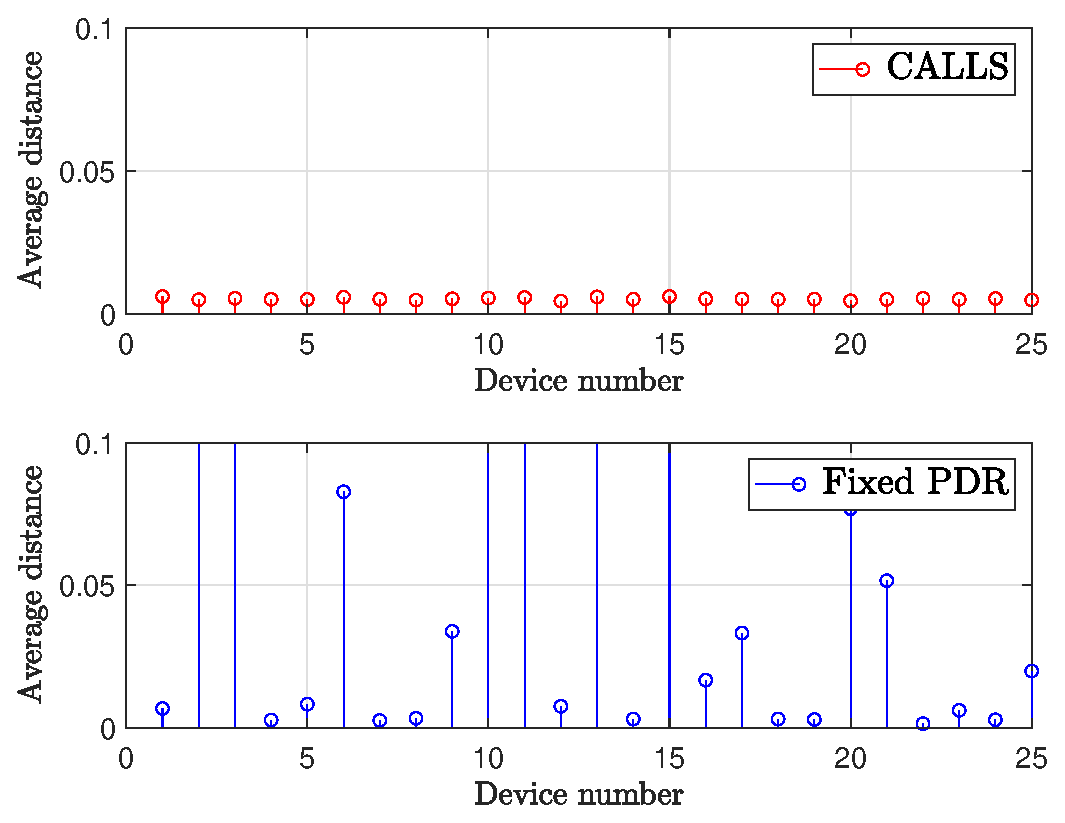
\includegraphics[width=.45\textwidth]{images/ip_dist.eps}
\caption{Average pendulum distance to center vertical for $m=25$ devices using (top) CALLS and (bottom) fixed-PDR scheduling with $\tau_{\max}= 1$ ms latency threshold. The proposed control aware scheme keeps all pendulums close to the vertical, while fixed-PDR scheduling cannot.}
\label{fig_ip_dist}
\end{figure}
%%

We present in Figure \ref{fig_ip_bar} the final capacity results obtained over all the simulations. We say that a scheduling method was able to successfully serve $m'$ devices if it keeps all devices within a  $|\theta_{i,k}| \leq 0.05$ error region for 100 independent simulations. Observe that the proposed approach is able to increase the number of devices supported in each case, with up to $1.5$ factor increase over the standard fixed PDR approach. Indeed, the proposed CALLS method is able to allocate the available resource in a more principled manner, which allows for the support of more devices simultaneously being controlled. 

%%%%%%
\begin{figure}
\centering
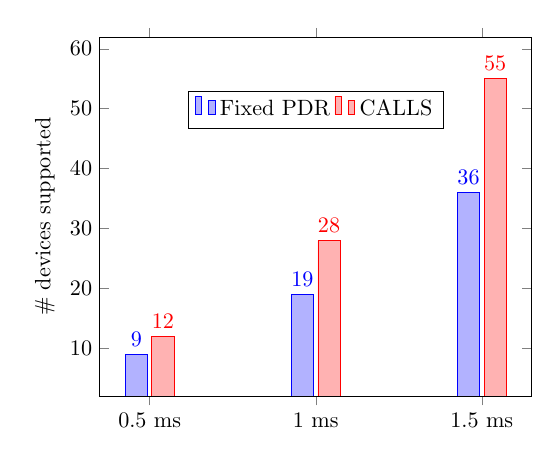
\begin{tikzpicture}[scale=0.8]
\begin{axis}[
    ybar,
    enlargelimits=0.15,
    legend style={at={(0.5,0.85)},
      anchor=north,legend columns=-1},
    ylabel={\# devices supported},
    symbolic x coords={0.5 ms,1 ms,1.5 ms},
    xtick=data,
    nodes near coords,
    nodes near coords align={vertical},
    ]
\addplot coordinates {(0.5 ms,9) (1 ms,19) (1.5 ms,36)};
\addplot coordinates {(0.5 ms,12) (1 ms,28) (1.5 ms,55)};
\legend{Fixed PDR, CALLS}
\end{axis}
\end{tikzpicture}
\caption{Total number of inverted pendulum devices that can be controlled using Fixed-PDR and CALLS scheduling for various latency thresholds.}
\label{fig_ip_bar}
\end{figure}
%%%%%%



\subsection{Balancing board ball system}

We perform another series of experiments on the wireless control of a series of balancing board ball systems developed by Acrome \cite{acrome}. In such a system, a ball is kept on a rectangular board with a single point of stability in the center of the board. Two servo motors underneath the board are used to push the board in the horizontal and vertical directions, with the objective to keep the ball close to the center of the board. The state here reflects the position and velocity in the horizontal and vertical axes, i.e. $\bbx_{i,k} := [x_{i,k}, \dot{x}_{i,k}, y_{i,k}, \dot{y}_{i,k}]$.  The input $\bbu_{i,k} = [v_x, v_y]$ reflects the voltage applied to the horizontal and vertical motors. As before, we apply a zeroth order hold on the continuous dynamics with a state sampling rate of $0.01$ seconds and linearize, thus obtaining the following dynamic system matrices,
%

\begin{align}\label{eq_control_orig}
\bbA_i =
\begin{bmatrix}
1 & 0.01 & 0 & 0 \\
0 & 1 & 0 & 0 \\
0 & 0 & 1 & 0.01 \\
0 & 0 & 0 & 1
\end{bmatrix},
\bbB_i =
\begin{bmatrix}
-0.0001 & 0\\ -0.02  & 0\\ 0 &-0.00008 \\ 0 & -0.01
\end{bmatrix}.
\end{align}
%
As before, we compute the control matrix $\bbK$ using standard LQR-control computation.

In Figure \ref{fig_bbb_dist} we show the results of a representative simulation of the control of $m=50$ balancing board ball systems with a latency bound of $\tau_{\max} = 10^{-3}$ seconds. Observe that, in this system, even with a large number of users the CALLS method can keep all systems very close to the center of the board, while the fixed PDR scheduler loses a few of the balls due to the agnosticism of the scheduler.

 To dive deeper into the benefits provided by control aware scheduling, we present in Figure \ref{fig_bbb_psr} a histogram of the actual  packet delivery rates each of the devices achieved over the representative simulation. It is interesting to observe that, in the CALLS method, the achieved PDRs are closely concentrated, ranging from 0.3 to 0.44. On the other hand, using a fixed PDR scheduling scheme, the non-variable rates are too strict for the low-latency system to support, and without control-aware scheduling the achieved PDRs range wildly from close to 0 to close to 1. In this case, some devices are able to transmit almost every cycle while others are almost never able to successfully transmit their packets. This suggests that, by using control aware scheduling, we indirectly achieve a sense of fairness across users over the long term. Further note that the PDRs required to keep the balancing board ball stable, e.g. 0.4, are relatively small. This is due to the fact that the balancing board ball features relatively slow moving dynamics, making it easier to control with less frequent transmissions. This is comparison to the inverted pendulum system, in which the pendulums were kept stable with PDRs in the range 0.6-0.75.

%%%%
\begin{figure}
\centering
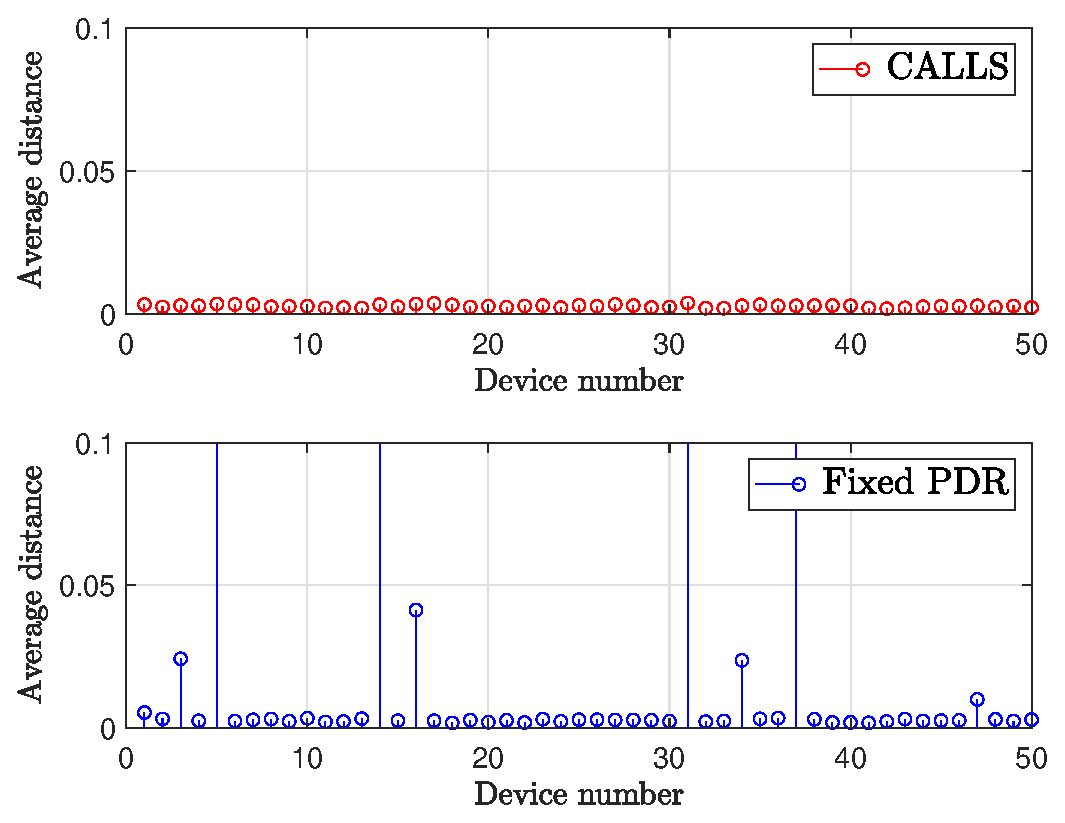
\includegraphics[width=.45\textwidth]{images/bbb_dist.eps}
\caption{Average ball distance to center for $m=50$ devices using (top) CALLS and (bottom) fixed-PDR scheduling with $\tau_{\max} =1$ ms latency threshold. The proposed control aware scheme keeps all balancing balls close to center, while fixed-PDR scheduling cannot.}
\label{fig_bbb_dist}
\end{figure}
%%

%%%%
\begin{figure}
\centering
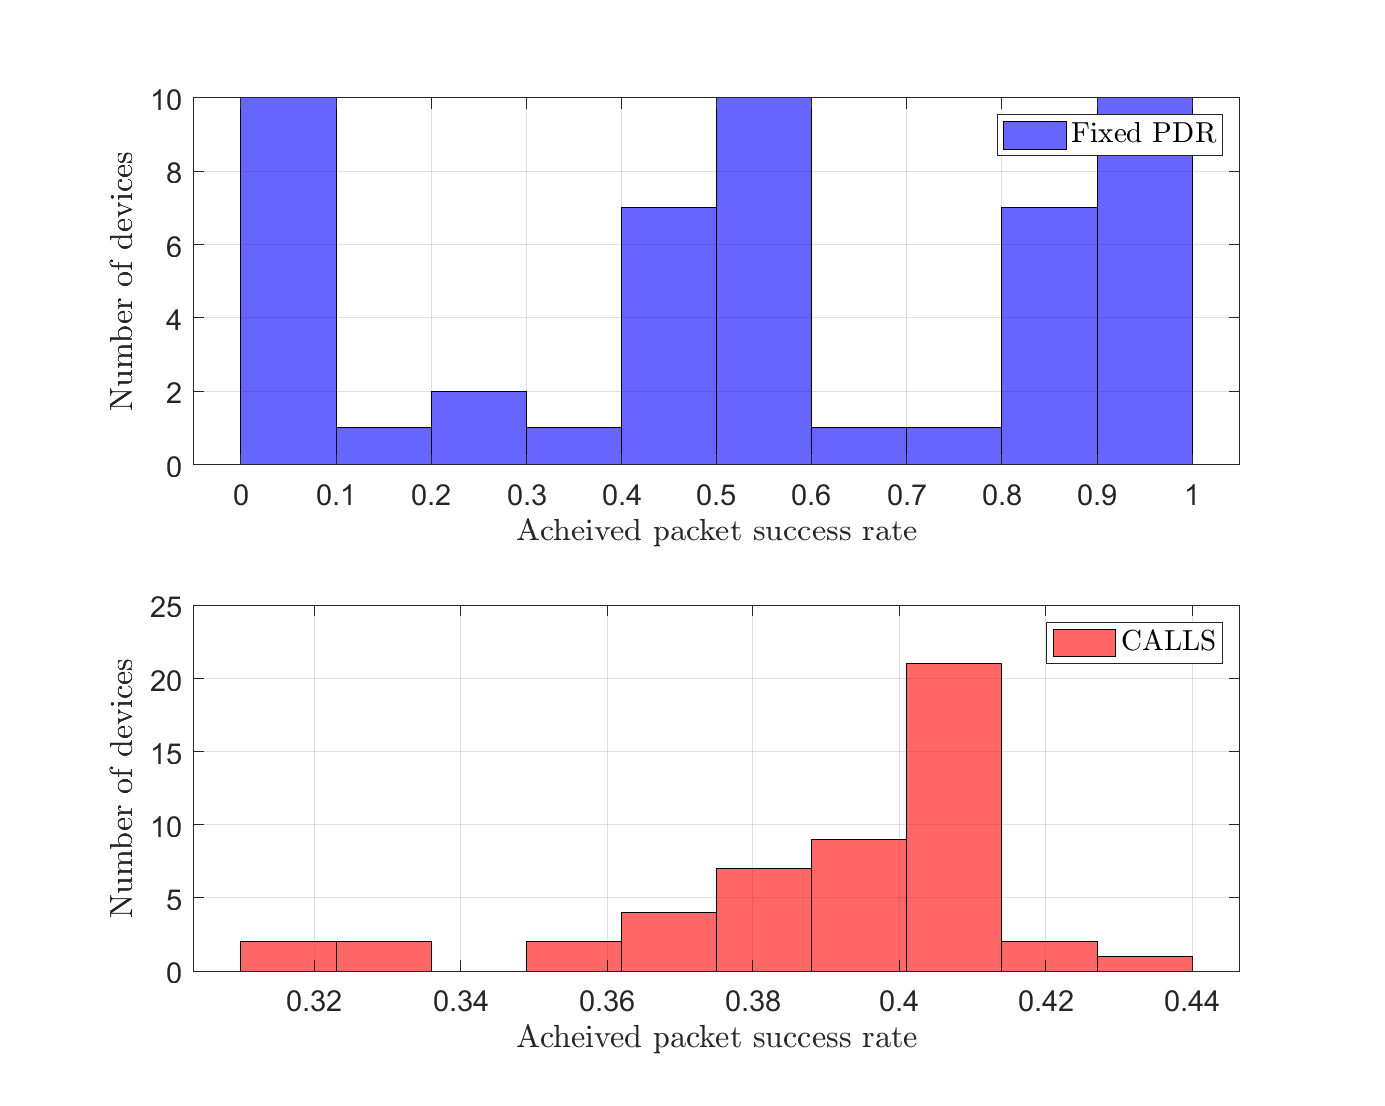
\includegraphics[width=.45\textwidth]{images/bbb_psr.eps}
\caption{Histogram of achieved PDRs in $m=50$ balancing board systems (top) CALLS and (bottom) fixed-PDR scheduling with $\tau_{\max} =1$ ms latency threshold. The proposed control aware scheme achieves similar PDRs for all devices, while the control agnostic scheduling results in large variation in packet delivery.}
\label{fig_bbb_psr}
\end{figure}
%%

We present in Figure \ref{fig_bbb_bar} the final capacity results obtained over all the simulations for the balancing board ball system. Observe that proposed approach increases the number of supported devices by factor of 2 relative to the standard fixed PDR approach. The even greater improvement here relative to the inverted pendulum simulations can be attributed to the slower dynamics of the balancing board ball, which allows for even more gains using control-aware PDRs due to the lower PDR requirements of the system.


%%%%%%
\begin{figure}
\centering
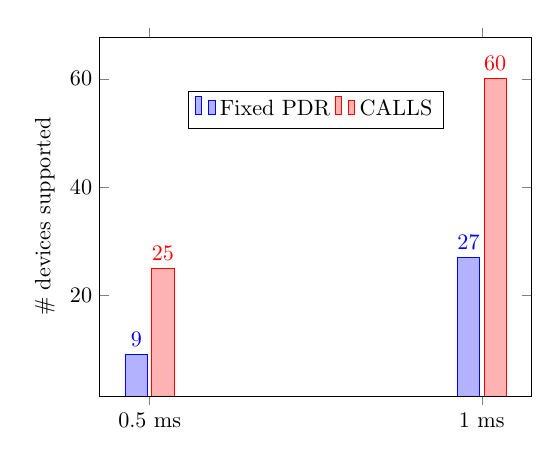
\begin{tikzpicture}[scale=0.8]
\begin{axis}[
    ybar,
    enlargelimits=0.15,
    legend style={at={(0.5,0.85)},
      anchor=north,legend columns=-1},
    ylabel={\# devices supported},
    symbolic x coords={0.5 ms,1 ms},
    xtick=data,
    nodes near coords,
    nodes near coords align={vertical},
    ]
\addplot coordinates {(0.5 ms,9) (1 ms,27)};
\addplot coordinates {(0.5 ms,25) (1 ms,60)};
\legend{Fixed PDR, CALLS}
\end{axis}
\end{tikzpicture}
\caption{Total number of balancing ball board devices that can be controlled using Fixed-PDR and CALLS scheduling for various latency thresholds.}
\label{fig_bbb_bar}
\end{figure}
%%%%%%


